\documentclass[a4paper, 11pt]{article}

\setcounter{tocdepth}{3}
\setcounter{secnumdepth}{3}

\usepackage{comment} % enables the use of multi-line comments (\ifx \fi) 
\usepackage{lipsum} %This package just generates Lorem Ipsum filler text. 
\usepackage{fullpage} % changes the margin
\usepackage[utf8]{inputenc}
\usepackage{gensymb}
\usepackage{graphicx}
\usepackage{booktabs}% http://ctan.org/pkg/booktabs
\usepackage{makecell}
\usepackage{tabularx}
\usepackage[table]{xcolor}
\usepackage{array}
\usepackage{wrapfig}
\usepackage{subcaption}
\usepackage{csquotes}
\usepackage{lscape}
\usepackage{afterpage}
\usepackage{geometry}
\usepackage{listings}

\geometry{a4paper, margin=1in}
\renewcommand{\figurename}{Abb.}
\newcommand{\code}[1]{\texttt{#1}}


\begin{document}
	
\title{Zusammenfassung Future IT-Infrastructure FS2018}
\author{Alex Neher}
\maketitle

\tableofcontents
\newpage

\graphicspath{{./Pictures/}}

\section{Netzwerk-Aspekte}
\subsection{VPN}
Ein VPN (Virtual Private Network) erlaubt es einem Benutzer, sich in ein Netzwerk 'einzuklinken', selbst wenn er physisch nicht am Standort des Netzwerks ist.

\subsubsection{Szenarien}
Es gibt verschiedenste Szenarien, in welchen ein VPN nützlich oder vonnöten ist. Einige davon sind z.B:
\begin{description}
	\item [Remote Access: ] Management eines Kundennetzwerks vom (Home-)Office aus, Zugriff auf HSLU-Ressourcen von zuhause. US-Netflix in der Schweiz schauen
	\item[Site-to-Site VPN: ] Verbindung zweier Netzwerke über einen verschlüsselten Tunnel. Von der Azure-Cloud ins EnterpriseLab, Verbindung zwischen zwei fixen IPs.
\end{description}

\subsubsection{Technologien}
Es gibt verschiedene Technologien, wie ein VPN aufgebaut sind. die zwei wichtigsten sind:

\begin{description}
	\item[SSL-VPN] Wird vor allem für \textbf{Remote Access} verwendet, da es mit einem relativ einfachen Setup verbunden ist. SSL-VPN läuft ausschliesslich über \textbf{Port 443 (HTTPS)}
	\item[IPSec-VPN] Dieses Protokoll wurde ursprünglich exklusiv für IPv6 entwickelt, ist nun aber auch auf IPv4 portiert worden. Es kann, wie das SSL-VPN ebenfalls für Remote Access eingerichtet werden, ist jedoch auch nützlich für Site-to-Site VPNs. IPSec-VPN wird als \textbf{wichtigstes VPN-Protokoll} heutzutage angeschaut.
\end{description}

\noindent Des weiteren gibt es noch diese zwei, veralteten und unsicheren Protokolle, die jedoch immer noch eingesetzt werden.

\begin{description}
	\item[PPTP (Point-to-Point-Tunneling Protocol): ] Basiert auf PPP \footnote{Point-to-Pont-Protocol}, ist jedoch veraltet und unsicher.
	\item[L2TP (Layer 2 Tunneling Protocol): ] Ist unverschlüsselt und vertraut darauf, dass wichtige Daten verschlüsselt werden, bevor sie getunnelt werden. Dementsprechend veraltet und unsicher.
\end{description}

\newpage

\subsubsection{IPSec}

\begin{wrapfigure}[13]{L}{0.55\textwidth}
	\centering
	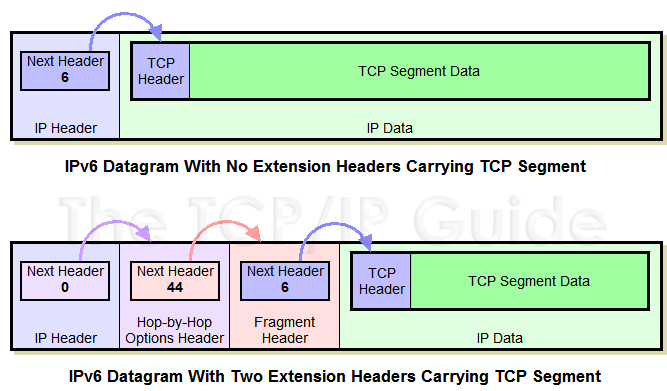
\includegraphics[keepaspectratio=true,height=10\baselineskip]{ipv6header.png}
	\caption{IPv6 unterstützt optionale Headers, die zwischen Payload und Header eingeschoben werden.}
	\label{fig:ipv6header}
\end{wrapfigure}


Da IPSec ursprünglich für IPv6 entwickelt wurde, unterstützt es dessen Konzept der \textbf{Header Extensions} (Abbildung \ref{fig:ipv6header}). IPv4 unterstützt jedoch \textit{keine} Header-Extensions! Bei IPv4 werden diese IPSec-Header einfach zwischen dem IP-Header und dem TCP/UDP-Header eingefügt.

\vspace{10px}

\noindent IPSec unterstützt die Verwendung des \textbf{AH} und/oder \textbf{ESP-Headers}.

\begin{description}
	\item[AH (Authentication Header): ] Die Authentizität des Datenursprungs ist sichergestellt.
	\item[ESP (Encapsulating Security Payload): ] Die Daten sind verschlüsselt
\end{description}

Die eingefügten Header beinhalten eingentlich nur eine \textbf{Sequenznummer} und einen \textbf{Index auf eine SA} (Security Association). Zudem wird das gesamte Paket noch mit einem \textbf{Hashwert} versehen, was jedoch dank NAT zu Problemen kommen kann, da das NAT die Authentizitäts-Garantie des Authentication Headers versaut.

\paragraph{Security Association} \mbox{} \\
Jedes IPSec Endgerät kann \textbf{beliebig viele} SA speichern. Eine SA ist grundsätzlich nur eine \textbf{Datenstruktur}, die (unter anderem) folgende Felder Informationen enthält:

\begin{description}
	\item[Authentifationsverfahren: ] Modi und Schlüssel falls AH verwendet wird.
	\item[Verschlüsselungsverfahren: ] Modi und Schlüssel, falls ESP verwendet wird.
	\item[Lebensdauer der SA und Schlüssel: ] Wie oft muss der VPN-Tunnel wiederhergestellt werden.
	\item[IP-Adresse der End-Netzwerk Gateways]
\end{description}

\noindent Beim Verbindungsaufwand wird diese SA aufgebaut. Dazu wird das \textbf{ISAKMP (Internet Security Association Key Management Protocol)} verwendet. 

\paragraph{ISAKMP}\mbox{} \\
 Das ISAKMP Protokoll besteht aus zwei Phasen:
\begin{description}
	\item[Phase 1: ] Ein \textbf{gemeinsamer Schlüssel} wird mit einem \textbf{erweiterten Diffie-Hellman-Verfahren} ausgehandelt (Bürgler lässt grüssen). Anschliessend werden die \textbf{Verschlüsselungs- und Hash-Protokolle ausgehandelt (nun in verschlüsselter Kommunikation)}. Dabei gibt es zwei verschiedene Modi: Im Main-Modus einigen sich beide Parteien auf die verwendeten Protokolle, während im Aggressiven Modus der Initiator 'seine' Protokolle vorgibt. Die Partner authentisieren sich via PSK, ihre Digitale Signatur, RSA oder El-Gamal.
	\item[Phase 2: ] Die SA wird nun aufgebaut und die weiteren Parameter für die IPSec-Verschlüsselung und den Tunnel werden ausgetauscht.
\end{description}

\newpage

\paragraph{Transport- vs. Tunnel-Mode}\mbox{} \\
\begin{wrapfigure}[16]{R}{0.6\textwidth}
	\centering
	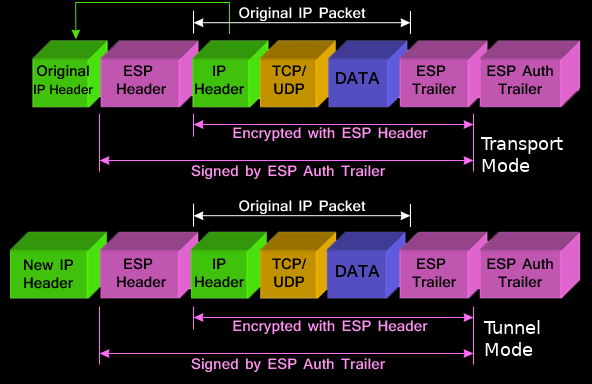
\includegraphics[keepaspectratio=true,height=12\baselineskip]{tunnelvstransport.png}
	\caption{Unterschied der Header zwischen dem Transport- und dem Tunnel-Mode}
	\label{fig:tunneltransport}
\end{wrapfigure}

Diese vorhin genannten weiteren Parameter sind z.B. ob der \textbf{Transport-} oder det \textbf{Tunnel-Modus} verwendet werden und ob \textbf{NAT-Traversal}\footnote{Ermöglicht es, das AH-NAT-Problem zu umgehen, indem die Pakete in UDP-Pakete encapsulated werden, die anschliessend über Port 4500 versendet werden..} erlaubt sein sollte.

Bei IPSec ist per Default der \textbf{Tunnel-Mode} eingestellt. In diesem Modus wird das \textbf{gesamte IP-Paket verschlüsselt}. IPSec nimmt es, verschlüsselt es, packt seinen IPSec Header davor und schickt es durch den Tunnel. Die allfälligen AH- und ESP-Header werden zwischen dem 'alten' IP-Header des zu verschlüsselnden Pakets und dem 'neuen' IP-Header des IPSec-Protokolls gepackt (Abbildung \ref{fig:tunneltransport} unten). 

Beim \textbf{Transport-Mode}, der hauptsächlich bei \textbf{End-to-End-Verbindungen)} wie z.B. Client zu Server eingesetzt wird, wird das IP-Paket durch \textbf{AH und/oder ESP-Header} verschlüsselt. Der IP-Header des Pakets wird beim Transport-Mode an den Anfang geschoben, gefolgt vom ESP (und evtl. AH-Header).

Transport-Mode wird meist mit einem anderen tunneling-Protokoll wie z.B. GRE gekoppelt. So wird der original Payload zuerst von GRP umschlossen, bevor IPSec das neue, umschlossene Paket durch den Tunnel schickt.

\paragraph{Verbindungsprobleme mit IPSec} \mbox{} \\
Es kann auch zu 'Show-Stopper' kommen beim Verbindungsaufbau mit IPSec, die verhindern, dass die Verbindung aufgebaut werden kann.

\begin{itemize}
	\item Der Initiator ist im Aggressiv-Mode und der Partner unterstützt die verlangten Protokolle oder den Aggressiv-Mode nicht (z.B. Android)
	\item Bei Remote Access VPN müssen IP-Adressen und weitere Informationen dynamisch übermittelst werden, die evtl. nicht untereinander kompatibel sind.
	\item Es gibt kein gemeinsames Set von Verschlüsselungs- oder Hash Algorithmen der beiden Seiten, bzw. die unterstützten Schlüssellängen sind nicht komptabiel.
\end{itemize}

In aller Regel sind Site-To-Site VPNs aber trotzdem möglich, solange die verwendeten Algorithmen bekannt und kompatibel sind.

\newpage

\subsection{WAN-Technologien}
\subsubsection{Definition}
WAN (Wide Area Network) sind \textbf{Netzwerk-Verbindungen} über \textbf{weite Distanzen}. Die Nutzen von WAN werden aufgeteilt in \textit{internet-basierte} und \textit{nicht-internet-basierte} Nutzen.
\vspace{10px}
  
\noindent  Internetbasierte Nutzen von WAN sind z.B. der Zugriff auf entfernte Ressoourcen über RDP oder Citrix, SSL-VPN oder Site-to-Site VPN via Internet.

\vspace{10px}

\noindent Nicht internet-basierte Nutzen von WAN sind z.B. Dark Fiber (Eine direkte Point-to-Point Verbindung zwischen zwei Standorten, die nicht am Internet hängt. Dark Fiber hat eine Reichweite von max 50km), LAN-Interconnect (Die Vereinigung zweier LANs über WAN), Private Lines oder Business VPN.

\subsubsection{Beurteilungskriterien}
Die Qualität von WAN-Verbindungen kann anhand verschiedener Kriterien gemessen werden.

\begin{description}
\item[Geschwindigkeit: ] Kann die Geschwindigkeit, die der ISP verspricht auch garantiert werden?
\item [Zuverlässigkeit: ] Wird die vereinbarte SLA zuverlässig eingehalten?
\item[Kosten: ] Hat der Service ein vertretbares Kosten/Nutzen Verhältnis?
\item[Redundanz: ] Garantiert der ISP eine Redundanz, falls eine Line unterbrochen wird?
\item[Konfiguration \& Management: ] Welche Möglichkeiten bietet der ISP?
\item[Provider/ISP: ] Welche Reputation hat der ISP? Wo ist er (vgl. Datenschutz), wie steht er wirtschaftlich da?
\item[Sicherheit: ] Wie schützt der ISP die Verbindung?
\end{description}

\subsection{IPv6}
IPv6 (Internet Protocol version 6) ist der Nachfolger des heute am weitesten verbreiteten Internet Protokoll IPv4. IPv4 wurde in den Anfangsjahren des Internets entwickelt und ware nie dazu gedacht, solche Mengen von Geräten zu managen, die heute am Internet hängen. Deshalb bietet es nur eine sehr begrenzte Anzahl von öffentlichen IP-Adressen an (4.3 Milliarden öffentliche IPs vs. ca. 11.2 Milliarden Geräte in 2018 \footnote{Quelle: https://www.gartner.com/newsroom/id/3598917})). Durch 'verschwenderische' Vergabe dieser IP-Adressen in den 90er Jahren und strukturelle Begebenheiten des Protokolls (subnetting als Beispiel), sind diese IPs heutzutage so gut wie erschöpft.

IPv6, das bereits 1998(!!) vom IETF standardisiert wurde, besteht aus einer 128bit langen hexadezimal-Zeichenfolge. Dadurch bietet das Protokoll \textbf{340 Sextilionen ($340 * 10^{36} $) Adressen}. Ausserdem bietet es weitere, nützliche Features wie eingebautes QoS, Mobile IP oder erweiterte automatische Konfigurationen der Netzwerkschnittstellen.

\subsubsection{Adressierung}
Eine IPv6-Adresse ist ein 128bit langer hexadezimal-String. Er wird in 8 Blöcke zu je 16bit unterteilt, die mit einem Doppelpunkt voneinander getrennt werden.

Da 128bit hexadezimal-Strings ein bisschen komplizierter sind wie 32bit dezimal-Nummern, gibt es einige Vereinfachungen und Guidelines, die das Arbeiten mit IPv6 vereinfachen sollen:

\begin{itemize}
	\item Falls ein Block mit Nullen startet, können diese weggelassen werden. Somit wird die Adresse \code{2001:0db8:0000:08d3:0000:8a2e:0070:7344} zu \code{2001:db8:0:8d3:0:8a2e:70:7344}
	\item Falls ein ganzer Block (oder mehrere aufeinanderfolgende) ausschliesslich aus Nullen besteht, so kann er ganz weggelassen werden. Das darf jedoch nur \textit{einmal} pro Adresse gemacht werden. \code{2001:0db8:0000:08d3:0000:8a2e:0070:7344} kann also abgekürzt werden \\
	zu \code{2001:db8::8d3:0:8a2e:70:7344}.
	\item Die letzten 4 Bytes (32bit) einer Adresse dürfen auch in Dezimal angegeben werden. Dies ist vor allem hilfreich, wenn IPv4 Adressen zu IPv6 Adressen umgewandelt werden. So kann die IPv4 localhost Adresse \code{127.0.0.1}, die eigentlich zu \code{0:0:0:0:0:ffff:7f00:1} wird, kann zur besseren Verständlichkeit auch als \code{0:0:0:0:0:ffff:127.0.0.1} (oder abgekürzt \code{::ffff:127.0.0.1}) geschrieben werden.
\end{itemize}

IPv6 unterscheidet im Gegensatz zu IPv4 nicht zwischen public und private IP Adressen. Diese Tatsache eigentlich auch das NAT obsolet, dessen einzige Aufgabe es war, mehrere private IPs zu einer public IP zu mappen. Stattdessen wird eine Subnetzmaske definiert (standartmässig 64bit). Die ersten 64bit identifizeren das Netzwerk und die restlichen 64bit identifizieren den Host in diesem Netzwerk. \code{2001:0db8:85a3:08d3:1319:8a2e:0370:7347/64} bezeichnet also den Host/die NIC \code{1319:8a2e:0370:7347} im Netzwerk. Analog wie im IPv4 bezeichnet \code{2001:0db8:85a3:08d3::/64} das gesamte Netzwerk (wie \code{192.168.0.0} in IPv4). 

\vspace{10px}

\noindent IPv6 Adressen werden zwar nicht in private und public Adressen unterteilt, jedoch wird zwischen verschiedenen \textbf{Adressarten} unterschieden:

\begin{description}
	\item[Link Local Unicast: ] Jede NIC/jeder Host, der IPv6-enabled ist, erhält automatisch eine Link Local Adresse. Sie wird \textbf{automatisch erstellt} und ist einzigartig für jeden Host und wird von dessen MAC-Adresse abgeleitet. Dieser Adresstyp wird \textbf{nicht geroutet}, soll heissen diese Adresse ist nur vom lokalen Subnetz aus anpingbar. 
	
	Mithilfe der Link Local Adresse wird z.B. Neighbour-Discovery gemacht. Ebenfalls wird normalerweise die Link Local Adresse des Routers als Gateway angegeben. 
	\item[Unique Local Unicast: ] Wie bereits erwähnt, arbeitet IPv6 nicht mit private und public Adressen, was NAT eigentlich obsolet macht. Jedoch ist es manchmal trotzdem wünschenswert, ausschliesslich im lokalen Netz zu kommunizieren. Unique Local Unicasts werden \textbf{ausschliesslich im eigenen LAN geroutet}, nicht jedoch im Internet.
	\item[Global Unicast: ] Dies ist die öffentliche IP des Host. Sie wird \textbf{im LAN und im Internet geroutet}.
	\item[Multicast: ] Multicasts werden verschickt, wenn die Link Local Adresse eines Hosts noch nicht bekannt ist. Sie sind das \textbf{Equivalent des IPv4 Broadcasts}.
	\item[Site Local Unicast: ] Vorgänger des Unique Local Unicasts, veraltet.
\end{description}

\subsection{Software Defined Networks}
\subsubsection{Momentaner State-of-the-Art}
Momentan werden Netzwerke \textbf{statisch} aufgebaut. Es wird geplant, getestet und anschliessend aufgebaut. Jede Änderung unterliegt dem \textbf{Change-Management} und muss zuerst genehmigt werden. Dasselbe gilt für virtualisierte Netzwerke wie z.B. VMWare-Cluster etc.).

%TODO


\section{Identity Management}

\subsection{Geschichtliches}
Als der Übergang von standalone-Systemen zu vernetzten Rechnersystemen stattfand, mussten Rechner plötzlich Informationen von anderen Rechnern im gleichen Netzwerk abfragen (wie z.B. IP- oder MAC-Adressen). Zudem mussten Benutzer in der Lage sein, Informationen/Dateien von anderen Rechnern abrufen und bearbeiten zu können. 

In den 8er Jahren kam schlussendlich die Idee auf, eine weltweite Datenbank mit allen vernetzten Rechnern aufzusetzen:

\paragraph{X.500} sollte folgende Eigenschaften besitzen:
\begin{itemize}
	\item Verteilte Informationen
		\subitem Jede Firma verwaltet seine Informationen selbst
		\subitem Jede Firma bestimmt, welche Informationen veröffentlicht werden, also von aussen zugänglich sind.
		\subitem Alle Firmen können auf veröffentliche Informationen von anderen zugreifen.
	\item Hierarchische Struktur mit objektorientierter Ausrichtung
		\subitem Vorwiegend geographisch aufgebaut.
		\subitem Hierarchie ist den konkreten Bedürfnissen anpassbar.
		\subitem Berechtigungen und Sicherheit sind auf jeder Hierarchiestufe definierbar.
	\item Hohe Verfügbarkeit
		\subitem Verteilte Datenbanken 
		\subitem Replizierte Datenbestände
		\subitem Verteilte Administration
\end{itemize}

Es stellte sich jedoch recht schnell heraus, dass eine einzige, globale Datenbank schlicht und einfach zu komplex ist. Zudem wurde X.500 praktisch nicht genutzt, höchstens als E-Mail-Adressen-Verzeichnis. Daraus folgt, dass es fast keine Produkte auf dem Markt gab, was die gesamte Situation nicht wirklich verbesserte. Aufgrund dessen erachteten es Betriebssystem-Hersteller auch nicht für nötig, native Unterstützung dieser Norm zu implementieren. $\rightarrow$ \textbf{X.500 starb recht schnell wieder aus.}

\newpage

\subsection{Begriffe}
\begin{wrapfigure}[10]{R}{0.4\textwidth}
	\centering
	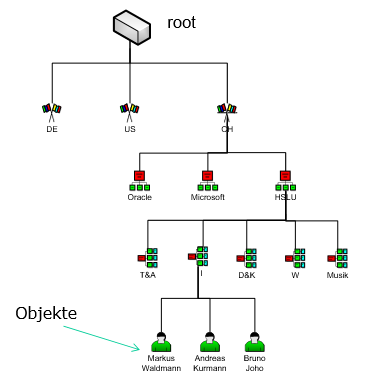
\includegraphics[keepaspectratio=true,height=10\baselineskip]{DIT.PNG}
	\caption{Beispiel eines DIT}
	\label{fig:dti}
\end{wrapfigure}
\paragraph{DIT - Directory Information Tree}\mbox{}\\
Der DIT wird verwendet, um Netzwerke darzustellen. Informationen werden hierarchisch dargestellt (siehe Abb. \ref{fig:dti} ). Im FAlle von X.500 war die Hierarchie Country (C) $\rightarrow$ Organization (O) $\rightarrow$ Organization Unit (OU). OUs halten weitere OUs oder Objekte, die mit einem Common Name adressiert werden. Am Beispiel von Abb. \ref{fig:dti} wäre ein Commmon Name 

\begin{lstlisting}
CN=Markus Waldmann, OU=Informatik, 
OU=I, O=HSLU, C=CH
\end{lstlisting}

\paragraph{DIB - Directory Information Base} \mbox{} \\


\section{Cloud Resources}

\section{Evalutation von Cloud-Services}

\section{Platform Trends}

\section{Betriebliche Aspekte}

\end{document}